\section{Quantization\buch{Chapter 2}}

\setArrayStretch{1.2}
\subsection{Quantization process\buchSeite{62}}
\begin{tabularx}{\textwidth}{|l|X|X|}
	\hline
	$R$			& full-scale range		& $R = Q \cdot 2^B$
	\\ \hline
	$B$			& bits					& $B = log_2 \left(\frac{R}{Q}\right)$
	\\ \hline
	$Q$			& quantization width	& $Q = \frac{R}{2^B}$
	\\ \hline
	$e$			& quantization error (quantization noise)	& $e_Q(nT) = x_Q(nT) -x(nT)$
	\\ \hline
	$e_{RMS}$	& root-mean-square error & $e_{RMS} = \frac{Q}{\sqrt{12}}$
	\\ \hline
	$r$	        & dynamic range         & $r = 20 log_{10}\left(2^B\right) \approx 6dB \cdot B$
	\\ \hline
	$SNR$		& signal-to-noise ratio (with uniform white noise)	& $SNR = 20 log_{10}\left(\frac{R}{Q}\right) = 6B\, dB$
	\\ \hline
	$\sigma_e^2$& average power / variance of quantization error & $\sigma_e^2 = E[e^2(n)] = \frac{Q^2}{12}$
	\\ \hline
\end{tabularx}


\subsection{Oversampling and noise shaping\buchSeite{66-70}}
\begin{tabularx}{0.75\textwidth}{|l|l|X|}
	\hline
	$L$	& oversampling ratio	& $L = \frac{f_s'}{f_s}$ with $f_s'$ as higher sampling rate
	\\ \hline
	$\Delta B$	& saved bits without noise shaping	& $\Delta B = 0.5 \cdot log_2(L)$ \\
				& saved bits with noise shaping		& $\Delta B = (p + 0.5) \cdot log_2(L) - 0.5 \cdot log_2\left(\frac{\pi^{2p}}{2p + 1}\right)$ \\
				& & $L = \left(\frac{2^{2\Delta B} \pi^{2p}}{2p+1}\right)^{\frac{1}{2p+1}}$	
	\\ \hline
	\multicolumn{3}{l}{p = order of the noise shaping filter}
\end{tabularx}


\textbf{Performance of oversampling noise shaping quantizers}:

\vspace{0.2cm}
\setArrayStretch{1.0}
\begin{tabularx}{0.65\textwidth}{|c|X|c|c|c|c|c|c|}
	\hline
	$p$	& $L$							& 4		& 8		& 16	& 32	& 64	& 128
	\\ \hline
	0	& $\Delta B \approx 0.5 \cdot log_2(L)$		& 1.0	& 1.5	& 2.0	& 2.5	& 3.0	& 3.5 \\
	1	& $\Delta B \approx 1.5 \cdot log_2(L) - 0.86$ & 2.1	& 3.6	& 5.1	& 6.6	& 8.1	& 9.6 \\
	2	& $\Delta B \approx 2.5 \cdot log_2(L) - 2.14$	& 2.9	& 5.4	& 7.9	& 10.4	& 12.9	& 15.4 \\
	3	& $\Delta B \approx 3.5 \cdot log_2(L) - 3.55$	& 3.5	& 7.0	& 10.5	& 14.0	& 17.5	& 21.0 \\
	4	& $\Delta B \approx 4.5 \cdot log_2(L) - 5.02$	& 4.0	& 8.5	& 13.0	& 17.5	& 22.0	& 26.5 \\
	5	& $\Delta B \approx 5.5 \cdot log_2(L) - 6.53$	& 4.5	& 10.0	& 15.5	& 21.0	& 26.5	& 32.0 \\
	\hline
\end{tabularx}
\resetArrayStretch

\vspace{0.2cm}
\begin{minipage}{0.3\textwidth}
  Oversampled quantization noise power, \textbf{without noise shaping.}
  
  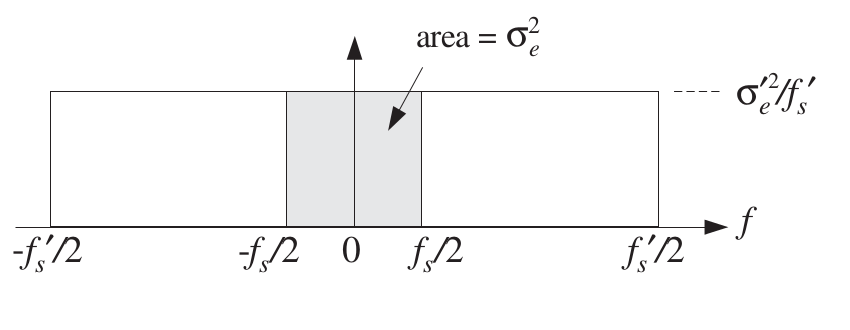
\includegraphics[width=\textwidth]{./picture/no_noise_shaping}
\end{minipage}
\hspace{0.1\textwidth}
\begin{minipage}{0.3\textwidth}
  Spectrum of oversampling \textbf{noise shaping quantizer}.
  
  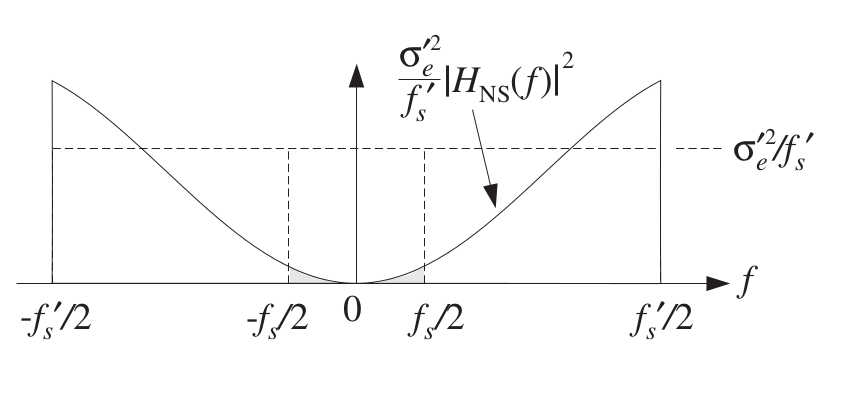
\includegraphics[width=\textwidth]{./picture/noise_shaping}
\end{minipage}


\subsection{D/A converters\buchSeite{71-73}}
\begin{tabularx}{\textwidth}{|l|X|l|l|}
	\hline
	\textbf{Name} & \textbf{Output calculation} & \textbf{Min} & \textbf{Max}
	\\ \hline
	natural binary
	& $x_Q = R(b_1 2^{-1} + b_2 2^{-2} + \ldots + b_B 2^{-B})$ 
	& $0$
	& $R-Q$
	\\ \hline
	offset binary
	& $x_Q = R(b_1 2^{-1} + b_2 2^{-2} + \ldots + b_B 2^{-B} - 0.5)$ 
	& $-\frac{R}{2}$ 
	& $\frac{R}{2} - Q$ 
	\\ \hline
	two's complement
	& $x_Q = R(\overline{b_1} 2^{-1} + b_2 2^{-2} + \ldots + b_B 2^{-B} - 0.5) \qquad (\overline{b_1}=1-b_1)$
	& $-\frac{R}{2}$ 
	& $\frac{R}{2} - Q$ 
	\\ \hline
\end{tabularx}


\subsection{A/D converters\buchSeite{75}}

\subsubsection{Successive Approximation Converters \buchSeite{76}}

\begin{center}
\begin{tabular}{|p{0.45\textwidth}|p{0.45\textwidth}|}
\hline
	\multicolumn{2}{|c|}{\textbf{Conversion algorithms}}\\
	\hline
	\textbf{Natural and offset binary}
		& \textbf{Two's complement}\\
	\hline
	if mode = rounding:\newline
		\hspace*{0.5cm} $y = x + \frac{Q}{2}$\newline
	else if mode = truncation:\newline
		\hspace*{0.5cm} $y = x$\newline
	for each $x$ to be converted, do:\newline
		\hspace*{0.5cm} initialize $\mathbf{b}=[0,0,\dots ,0]$\newline
		\hspace*{0.5cm} for $\mathbf{i}=1,2,\dots , B$ do:\newline
		\hspace*{1cm}$b_i = 1$\newline
		\hspace*{1cm}$x_Q = \text{dac}(\mathbf{b}, B, R)$\newline
		\hspace*{1cm}$b_i = u(y-x_Q)$
		& if mode = rounding: \newline
		\hspace*{0.5cm} $y = x + \frac{Q}{2}$ \newline
		else if mode = truncation: \newline
		\hspace*{0.5cm} $y = x$ \newline
		for each $x$ to be converted, do:\newline
		\hspace*{0.5cm} initialize $\mathbf{b}=[0,0,\dots ,0]$\newline
		\hspace*{0.5cm} $b_1 = 1- u(y)$ \newline
		\hspace*{0.5cm} for $\mathbf{i}=2,3,\dots , B$ do:\newline
		\hspace*{1cm}$b_i = 1$\newline
		\hspace*{1cm}$x_Q = \text{dac}(\mathbf{b}, B, R)$\newline
		\hspace*{1cm}$b_i = u(y-x_Q)$\\
	\hline
\end{tabular}
\end{center}

\subsection{Analog and digital dither\buchSeite{84-86}}
Dither is a small white noise signal that is added to the input signal befor quantization. The variance of the noise is $\sigma_v^2$ and the variance of the quantization is $\sigma_e^2$. The total variance is :

\[ \sigma_{\epsilon}^2 = \sigma_e^2 + \sigma_v^2 =\frac{1}{12}Q^2+\sigma_v^2\]

\begin{equation*}
	\sigma_{\epsilon}^2 = 
	\begin{cases}
		\frac{Q^2}{12} & \text{undithered} \\
		\frac{2Q^2}{12} & \text{rectangular dither} \\
		\frac{3Q^2}{12} & \text{triangular dither} \\
		\frac{4Q^2}{12} & \text{gaussian dither} \\
	\end{cases}
\end{equation*}

Goal of the dither is to eliminate quantization distortion and granulation and force the quantization error to look more
like white noise.
